\documentclass{report}

%\usepackage{pslatex}
%\usepackage{apa}
%\usepackage{apacite}
\usepackage{graphicx}
%\usepackage{float}
\usepackage{amssymb,amsmath} 
%\usepackage{helvet} 
%\usepackage[OT1]{fontenc}
\usepackage{helvet}
\renewcommand{\familydefault}{\sfdefault}
%\usepackage[small]{caption}

\setlength{\parindent}{0pt}
\setlength{\parskip}{2ex plus 0.5ex minus 0.2ex}

\title{Functional Adaptive Sequential Testing \\ (FAST a.1.0)}

\author{Ed Vul, Don MacLeod}


%outline



\begin{document}

\maketitle

FAST is a Matlab toolbox for efficiently estimating thresholds in behavioral experiments.  The primary role of FAST is to determine what is the most informative next trial.

FAST allows you to do the following:
\begin{enumerate}
\item Estimate thresholds and width/slope.
\item Estimate thresholds as a function of some other stimulus parameter
\item Choose optimal stimuli for different estimation goals.
\item Shrink, move, and otherwise adaptively alter the search parameter space.
\item Implement elaborate stopping rules.
\item Set priors on all of your parameters
\end{enumerate}

FAST can do many things; however, the more bells and whistles there are, the more complicated the interface. We�ve tried to make the additional complexities of FAST invisible and unnoticeable to those using its basic functions, but at points, some aspects of basic usage might be confusing because they also have to serve more complicated uses.


\tableofcontents

\clearpage

\section{Overview}

FAST staircases are designed to estimate thresholds.  They are most useful for estimating thresholds with the end goal of describing how these thresholds change as a function of some other variable.  For instance,  estimating contrast thresholds at different spatial frequencies to estimate the contrast sensitivity function.

To use FAST in an experiment, you have to 
\begin{enumerate}
\item Create a FAST structure, 
\item Choose a stimulus
\item Update the FAST structure with the response and stimulus values for the particular trial.
\item Repeat 2-3 until stopping.
\end{enumerate}

Each of these steps can be very simple, or very complicated, depending on what you want to get out of FAST.  We will describe the basic usage, and then describe the various ways in which these three steps can be customized and complicated to achieve specific goals.

\section{Framework}
We will describe the general FAST framework using the contrast sensitivity function (CSF) as an example:\\
Let $x$ be the spatial frequency\\
Let $y$ be the contrast\\
Let $p$ be the probability of responding `Yes' on the detection task.\footnote{Although forced-choice experiments are more commonly used for estimating the CSF, we will consider a `Yes'/`No' detection task for now because of its simplicity in not requiring the rescaling of response probabilities.  In practice, this is a less useful task because of response bias.}

Our goal is to estimate $p$ as a function of $x$ and $y$. We will do so by factoring the problem by assuming that
\begin{equation}
p(x,y) = \Psi(y | y^*(x), \Theta_{\Psi}) ,
\end{equation}
where $\Psi $ is a \emph{psychometric function} with slope and lapse parameters given by $\Theta_{\Psi}$; $y$ is the contrast; and $y^*(x)$ is the threshold detection contrast at spatial frequency $x$ --- thus, we are assuming that $x$ has an effect on the probability of detection only by altering the threshold along $y$.  

We can then specify 
\begin{equation}
y^*(x)=F(x, \Theta_{F}) ,
\end{equation}
where $F$ is some function with parameters  $\Theta_{F}$ that is adopted as a working approximate description of the relation of $x$ to the threshold value of $y$ --- we call this the \emph{threshold function}.

So to complete the contrast sensitivity example we can say that the psychometric function is a Weibull
\begin{equation}
p=\Psi(y | y^*(x), \Theta_{\Psi}) = 1-\exp\left({-\frac{y}{y^*(x)}^{\Theta_{\Psi}}}\right)
\end{equation}
and the threshold function is obtained from Mannos \& Sakrinson (1974)"
\begin{equation}
y^*(x)=F(x, \Theta_{F}) = \Theta_F(1) \left({\Theta_F(2) + \frac{x}{\Theta_F(3)}}\right) * \exp\left({-\frac{x}{\Theta_F(3)}^{\Theta_F(4)}}\right)
\end{equation}

Using this formulation, we can more efficiently sample points in the $x$, $y$ plane to determine the parameters of $\Psi$ and $F$.

\section{Installation}

Unpack/copy the FAST directory with its subdirectory structure intact (innards, funccurve, funcpsych) into some path (e.g., the Matlab toolbox path, but that's not necessary)

Go into that directory in Matlab and run setup.m.  This will add FAST to the Matlab path and will attempt to create a FAST structure, if all is well it should print ``Path setup completed." when it is done.

\section{Basic Usage: Getting Data}

Again, to use FAST in an experiment, you have to 
\begin{enumerate}
\item Create a FAST structure, 
\item Choose a stimulus
\item Update the FAST structure with the response and stimulus values for the particular trial.
\item Repeat 2-3 until stopping.
\end{enumerate}

\subsection{What you need to know}

To use FAST you need to know some basics about what task you are running and how the stimulus parameters relate to one another:

{\bf What is the task? (yes/no, matching, nAFC?)}\\
This will determine the range of the psychometric function by specifying what the level of chance guessing is, etc.  So you need to know whether the experiment is a detection (yes/no), matching (too much/too little), or alternative forced-choice (right/wrong).  If it is an alternative forced choice, how many alternatives are there (2, 4, etc.)?\\
This task distinction determines how we rescale the psychometric function to account for chance guessing and lapse rates.

{\bf What is the scale of the $y$ dimension? (linear or logarithmic?)}\\
This amount to asking how the experiment is parameterized, and what are the possible values of the $y$ parameter of the stimulus. Are $y$ values only positive, like luminance contrast, for which negative values are meaningless? If so, $y$ is logarithmic.  Or are they effectively unbounded, meaning that they can take on positive and negative values (like the logarithm of luminance contrast)?  If so, the $y$ variable is linear.  If we describe contrast as log(contrast) then $y$ will be between -infinity and infinity, and will thus be linear.  Simply put, the question is: can $y$ be negative?  If so, it is on a linear scale; if it is bounded at 0, then it is a logarithmic scale.\\
This linear/logarithmic distinction will determine how to treat $y$ in the psychometric function.  For basic usage, we always use the Logistic psychometric function and appropriately transform the $y$ variable within FAST --- more advanced users can specify one of many alternate psychometric functions, or even add their own.

{\bf What is the threshold function that connects the $x$ stimulus variable to the $y$ stimulus variable?}\\  
For example, when doing a simple single-$x$-value threshold estimation, the appropriate function is \verb#funcVal# which says that $y^*(x) = c$: the threshold is constant $c$ for all $x$.  \\
For actual two-dimensional experiments, some functional form must be assumed, which may be as simple and generic as a line with some slope and intercept (\verb#funcLine#), as complicated as an $n$th degree polynomial (\verb#funcPoly#), or as specific as the contrast sensitivity function outlined earlier (\verb#funcCSF#).  A number of generic functions are included with FAST, and adding custom threshold functions is quite easy. 

{\bf What is a plausible range for parameter values?}\\
You should provide an estimate of the parameters of the threshold function (e.g., for \verb#funcVal#, an estimate of the threshold;  for \verb#funcLine# an estimate of the slope and intercept, etc.), as well as an estimate of the width/slope of the psychometric function.\\
In practice, there are two ways to specify the initial guess about the values of a parameter: as a range, or as a Gaussian (or Log-Normal) prior.  For basic usage, specifying a range is the easiest course of action, and a ``prior" is inferred from the set range.  

\subsection{Example: \\Basic threshold estimation in a detection task}

As a simple example, lets pretend we are running a simple detection experiment (lets say we present a gabor with contrast $y$ and a fixed spatial frequency and we ask subjects to press a button if they detect it $r=1$ and another button if they did not detect it $r=0$).  

{\bf 1. Setting up the FAST structure}

We will set up the FAST structure using the simple \verb#fastStart# function, which is run as follows:

\begin{verbatim}
myfast = fastStart(nchoice, CurveFunc, CurveParams);
\end{verbatim}

\verb#nchoice# is an integer specifying the sort of task being done, in our case \verb#nchoice = 1#, meaning ``detection" (0 corresponds to matching, and values 2 and above correspond to n-alternative forced choice tasks).

\verb#CurveFunc# is a string specifying the name of the threshold function --- in our case \verb#'funcVal'#, for a single threshold, with one parameter: the translation of the psychometric function.  FAST will assume that we want to use the default, Logistic, psychometric function.

\verb#CurveParams# is a cell array specifying the initial estimates of each parameter of \verb#CurveFunc#, and the width/slope of the psychometric function. In our case, there is only one parameter for \verb#CurveFunc#: the constant threshold.  Since we are using the default logistic function, we will consider $log_{10}(contrast)$ to be our stimulus parameter, so we will guess that the the $log_{10}$ threshold contrast will lie somewhere between 0 and 2.  There is one parameter (slope) for the default (logistic) psychometric function, which we will loosely estimate to be between 0.001 and 1 so, \verb#CurveParams={[0 2], [0.001 1]}#

Thus initializing the FAST structure in this case will be achieved with the command:

\begin{verbatim}
myfast = fastStart(1, 'funcVal', {[0 2], [0.001 1]});
\end{verbatim}

So we�ve set up a single threshold estimation where we estimate the threshold to be between 0 and 2 log-units, with a detection task (1-AFC) using a Logistic function (default) with width/slope (discrimination threshold for the logistic) estimated to be between 0.001 and 1 unit.

{\bf 2. Choosing a stimulus value}

The simplest way to choose a stimulus value would be simply to do our best to present a stimulus at the 50\% detection threshold --- analogous to running a 1-up, 1-down staircase.  For this we can use the default settings of the \verb#fastChooseY# function\footnote{In actuality, the default setting for fastChooseY is to present a stimulus at either 40\%, 50\% or 60\% (one of these is randomly selected, and then re-scaled to the appropriate psychometric range for the task at hand), this is designed to improve the estimation of the slope as well as the threshold.}:

\begin{verbatim}
y = fastChooseY(fastStruct, xs);
\end{verbatim}

In our case, \verb#xs# is meaningless (since we are estimating a constant threshold), so we may as well fix it to 0; and \verb#fastStruct# is the FAST structure we just created (\verb#myfast#).

\begin{verbatim}
y = fastChooseY(myfast, 0);
\end{verbatim}

{\bf 3. Update FAST}

After we present a trial to the subject we need to update our parameter estimates so that we can use this trial's information to inform the next trial.  We do so with the \verb#fastUpdate# function:

\begin{verbatim}
fastStruct = fastUpdate(fastStruct, [x y r]);
\end{verbatim}

In our case, assuming we just presented a detection trial with contrast \verb#y#, then \verb#fastStruct# is \verb#myfast#; \verb#x# is 0; and \verb#r# is either 0 (if the stimulus was not detected), or 1 (if the stimulus was detected) --- let's say the stimulus was detected, so we update the FAST structure with:

\begin{verbatim}
myfast = fastUpdate(myfast, [0 y 1]);
\end{verbatim}

We will iterate steps 2 and 3 until we are satisfied (deciding when we ``are satisfied" may be done by fixing the number of trials for now, later we will discuss how to use confidence in parameter values to decide when to stop).

\subsection{Example: \\Basic estimation of a hyperbolic decay in a matching task}

Lets pretend we are running a simple experiment on delay discounting. We present subjects with an alternative: ``would you rather have \$$v_n$ now or \$$v_d$ in $x$ days?" When subjects say they prefer the immediate amount, $r=1$: we are offering them too much for the immediate reward; when the prefer the delayed amount $r=0$, we are offering them too little for the immediate reward.  Thus, we are running a sort of cognitive ``matching" experiment, to find the equivalence point of immediate and delayed rewards given a particular delay.  Our goal is to estimate the hyperbolic discounting rate.

{\bf 1. Setting up the FAST structure}

We will set up the FAST structure using the simple \verb#fastStart# function, again.  This time

\verb#nchoice# will be 0 for matching.

\verb#CurveFunc# will be the commonly accepted hyperbolic discounting function:
\begin{equation}
v_n = v_d/(1 + a x) ,
\end{equation}
where $v_n$ is subjectively equivalent in value as $v_d$ in $x$ days.  Thus we will use the \verb#'funcHyperbolic'# function to connect delay to value. The hyperbolic function in FAST defines $y^*(x) = 1/(1+ a x)$, so this tells us how to scale the delayed reward ($v_d$) to obtain the immediate reward ($v_n), to compute both portions  to  presenting the stimulus.  Thus $y = v_d / v_n$, $x$ is the delay, and $r$ is preference for the current reward or the delayed reward.

\verb#CurveParams# is the parameter cell array, we will estimate the hyperbolic discounting rate to be between 0.001 (it takes 1000 days for the value of the delayed amount to decrease by a factor of two), and 1 (it takes one day for this to happen); we will use the same psychometric slope parameters as in the previous section.  Thus: \verb#CurveParams={[.001 1], [0.001 1]}#

We initialize the FAST structure:

\begin{verbatim}
myfast = fastStart(1, 'funcHyperbolic', {[.001 1], [0.001 1]});
\end{verbatim}

Thus, we�ve set up a structure to estimate the hyperbolic discounting rate for a particular subject by adaptively testing in a ``cognitive matching" experiment.

{\bf 2. Choosing a stimulus value}

In this example, to choose a $y$ stimulus value we need to specify $x$, the length of the delay.  So we can choose a random integer delay value ($x$) between 1 and 100 days.  We will choose a particular delayed reward amount $v_d$; for the sake of convenience we will choose this to be \$10 (we can also randomly alter $v_d$ on each trial, but the delay discounting parameter is known to vary with the magnitude of rewards, so let's not introduce that sort of noise here):

\begin{verbatim}
x = randi(100);
v_d = 10;
\end{verbatim}

Then we use \verb#fastChooseY# to obtain a discounting proportion ($y$) for delay $x$, and  use these to obtain our guess about the immediate reward ($v_n$) that would subjectively match the delayed reward (in other words, the immediate value that will be close to the subject's indifference point.

\begin{verbatim}
y = fastChooseY(myfast, x);
v_n = v_d * y;
\end{verbatim}

Thus, FAST is internally estimating the hyperbolic discounting rate, and predicting the proportional discounting at particular delays ($y$), while we present the subject with dollar values ($v_n$ and $v_d$).

{\bf 3. Update FAST}

After we present a trial to the subject and obtain a preference ($r=1$ for immediate, $r=0$ for delayed) we need to update our parameter estimates.  Since we set up the internal representation for FAST to be of unscaled discounting proportion (rather than dollar values) we must update with the discounting proportion as the $y$ value::

\begin{verbatim}
fastStruct = fastUpdate(fastStruct, [x y r]);
\end{verbatim}

There --- we have completed a trial, and are ready to repeat as many more as necessary.

\section{Basic Usage: Obtaining results}

For the sake of the examples below, I (Ed Vul) ran in about 50 trials of the very simple discounting experiment described in the previous section.  The code for this experiment can be seen here:

\begin{verbatim}
clear all
close all

myfast = fastStart(1, 'funcHyperbolic', {[.001 1], [0.001 1]});

i = 0;
while i < 50
    x = randi(100);
    v_d = 10;
    y = fastChooseY(myfast, x);
    v_n = v_d * y;
    
    r = input(sprintf('$%2.2f now [1] or $%2.2f in %d days [0]', v_n, v_d, x));
    
    myfast = fastUpdate(myfast, [x y r]);
    i = i+1;
end

save ~/Code/dd_test.mat;
\end{verbatim}

\subsection{Viewing data and function fits}

To view the current data and function fits one can run the command \verb#fastPlot#:

\begin{verbatim}
fastPlot(myfast);
\end{verbatim}

The output of this command run on the hyperbolic data can be seen in Fig. \ref{fig:fastplot}.  Please see figure caption for a detailed description.  Effectively, this command shows the current data -- the history of trials, and responses, the best function fit to these data, as well as a few other plots to validate the model fit.


\begin{figure}
\begin{center}
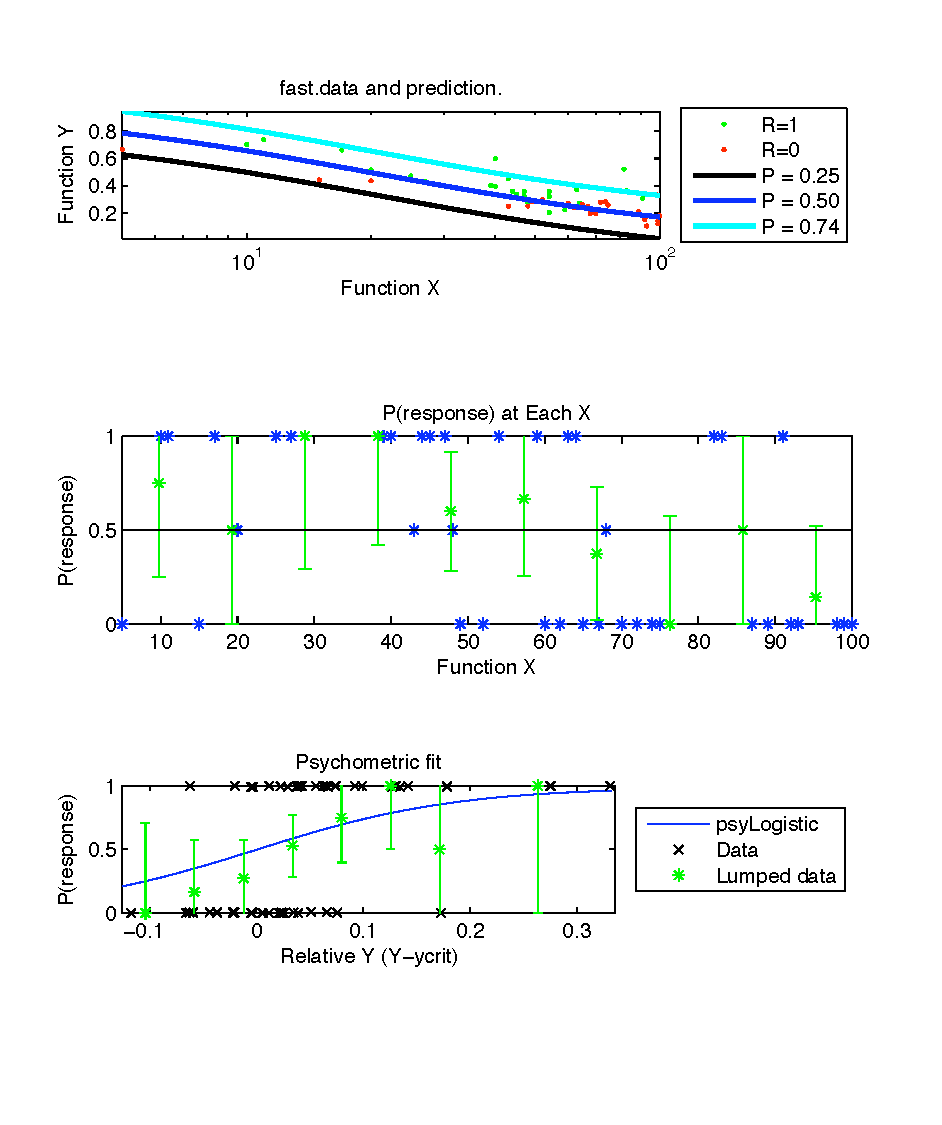
\includegraphics[scale=0.75]{figures/fastPlot-ed-hyperbolic.pdf}
\caption{
\label{fig:fastplot}
The output of the fastPlot command on the hyperbolic discounting ``experiment". \\
 \emph{Top: }A summary of all the data (distinct points -- green for $r=1$ (immediate preferred), red for $r=0$ (delayed preferred) as a function of $x$ (delay in days) and $y$ (the discounting proportion; see text).  The three lines represent the model posterior predictive fits for the 25\%, 50\% and 75\% threshold function. \\
 \emph{Middle: }Proportion of $r=1$ and $r=0$ responses as a function of $x$; this is a crude way to test for systematic deviations from the fit of the model, in our case it seems that there are no systematic deviations, meaning that a hyperbolic function fits these data well; however, we are only working on about 50 trials).  \\
 \emph{Bottom: } The fit of the psychometric function to the data scaled appropriately by the factoring out the modulations in $x$ -- in other words, the psychometric function of $y - y^*(x)$.}
\end{center}
\end{figure}


\subsection{Obtaining parameter estimates and confidence intervals}

To view current parameter estimates and obtain specific confidence intervals by running the command,
\begin{verbatim}
estimate = fastEstimate(myfast);
\end{verbatim}

This simple line command, (a) a figure as shown in Fig. \ref{fig:fastestimate}, which contains a graphical illustration of posterior probabilities over parameter values from the hyperbolic discounting example (see figure caption for details), and (b) numerical estimates of these parameters as well as confidence intervals.

The output of this command produces the following output structure:

\verb#estimate.islog# indicates whether the parameters are treated as logarithmic (and thus log-normal posteriors intervals are estimated), or if they were treated as linear (thus using normal posteriors)

\verb#estimate.marg# contains the means (\verb#estimate.marg.mu#) and standard deviations (\verb#estimate.marg.sd#) for either a log-normal or a normal marginal distribution, depending on the ``islog" setting for that parameter.  \verb#estimate.marg.mean# contains the marginal mean in the native scale for that parameter, and \verb#estimate.marg.quantiles# contains the native-scale quantiles for each parameter (default quantiles are 0.025, 0.1, 0.5, 0.9, 0.975, but these can be customized as needed, see section \verb#!!#).

For now, the only other relevant component of \verb#estimate# is \verb#interp#, which displays, among other things, the non-parametrically interpolated quantiles of the marginal for each parameter.  

For the present example, these outputs are:

\begin{verbatim}
estimate = 
         islog: {[1]  [1]}
          marg: [1x1 struct]
        margXC: [1x1 struct]
         gauss: [1x1 struct]
    latticeMax: {[0.0435]  [0.0550]}
        interp: [1x1 struct]

>> estimate.marg

ans = 

           mu: [-1.2916 -0.9896]
           sd: [0.1602 0.3425]
         mean: {[0.0511]  [0.1024]}
    quantiles: {[0.0248 0.0319 0.0511 0.0820 0.1053]  
                [0.0218 0.0373 0.1024 0.2814 0.4805]}
    
>> estimate.interp

ans = 

        pvals: {[1x21 single]  [1x21 single]}
      llhvals: {[1x21 single]  [1x21 single]}
    quantiles: {[0.0377 0.0409 0.0473 0.0552 0.0601]  
                [0.0373 0.0485 0.0896 0.3324 0.9236]}
\end{verbatim}

\begin{figure}
\begin{center}
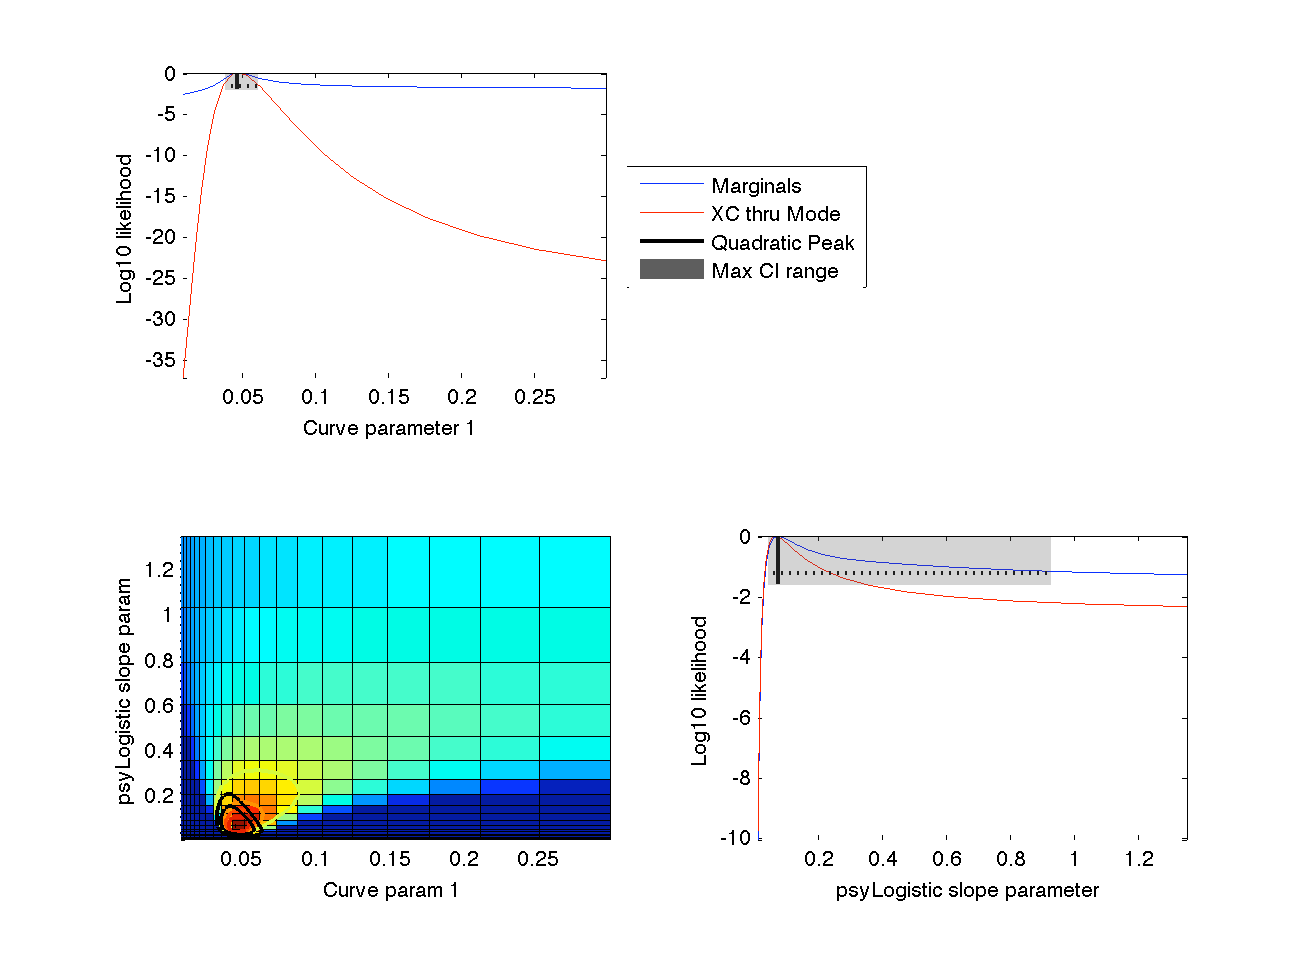
\includegraphics[scale=0.5]{figures/fastEstimate-ed-hyperbolic.pdf}
\caption{
\label{fig:fastestimate}
The output of the fastEstimate command on the hyperbolic discounting ``experiment". \\
 \emph{Top: }The marginal distribution of the hyperbolic discounting parameter, along with its confidence interval.  \\
 \emph{Bottom-Left: }The joint distribution of the hyperbolic discounting parameter (x axis) and the Logistic slope parameter (y-axis); hotter colors correspond to greater log-posterior.  Confidence ellipses are displayed as well.\\
 \emph{Bottom-Right: }Marginal log-posterior of the Logistic slope parameter, along with its confidence interval.}
\end{center}
\end{figure}

\section{Advanced use}

Now we will outline the various ways in which each step of a FAST experiment may be customized.  The steps, again, are:

\begin{enumerate}
\item Create a FAST structure, 
\item Choose a stimulus
\item Update the FAST structure with the response and stimulus values for the particular trial.
\item Repeat 2-3 until stopping.
\end{enumerate}

\subsection{Create FAST structure}

The complete FAST initialization is done through the function \verb#fastFull#, with a number of customizations:

\begin{verbatim}
myfast = fastFull(nchoice, funccurve, funcpsych, parameters [, xylims]);
\end{verbatim}

{\bf nchoice}

As described in the earlier section, nchoice specifies the task of the experiment:\\
0 corresponds to a matching experiment,\\
1 corresponds to a detection (yes / no) experiment, and\\
2+ corresponds to an n-AFC experiment.\\
This is unchanged in the advanced initialization.

{\bf funccurve}

This parameter is also unchanged, it takes as a string the name of the function (which can be found in the \verb#funccurve# directory of the FAST tree), for instance \verb#'funcVal'#, or \verb#'funcCSF'#.  See \verb#!!# for a list of default functions that are built in, as well as instructions about how to make new threshold functions.

{\bf funcpsych}

This parameter specified the psychometric function to be used in the experiment, by default in \verb#fastStart# this parameter was set to \verb#'psyLogistic'#, but a number of different functions may be specified.  See \verb#!!# for a list of included psychometric link functions that are built in by default.  New psychometric functions are harder to write (as they involve specifying the forward and inverse computations of the function), but it is still possible with some thought and mathematical effort.

{\bf parameters}

The parameters input specifies the estimates for each parameter of \verb#funccurve# and \verb#funcpsych#.  It takes the general form of:
\begin{verbatim}
{[funccuve param 1], ... [funccurve param n], [funcpsych slope]}
\end{verbatim}
However, there are three different ways to specify an initial estimate for the parameters:

\verb#[min max]#\\
This is the simplest method which specifies the minimum and maximum values of the plausible range for this parameter.  FAST figures out if this parameter should be treated as logarithmic or linear based on the range covered by the min and max: If either of these is negative, the parameter is linear; if both are positive, and they span a range of more than 1 order of magnitude\footnote{in fastSetting.m, this value is coded as ORDERMAGTHRESH: it is 1 by default}, then they are deemed logarithmic; if they are positive and span less than 1 order of magnitude, they are deemed to be linear.  The prior defaults to a uniform over this range, given this scaling.

\verb#[S v1 v2]#\\
This method specifies a normal (or log-normal) prior over the parameters.  $L$ indicates whether the parameter is distributed according to a normal, log-normal, or uniform distribution. \\
$S=1$ means that the parameter is distributed according to a log-normal distribution, in other words, $log_{10}(parameter)$ is distributed according to a normal distribution with mean=$v1$ and standard deviation equal to $v2$.  Thus, $v1=\mu$ and $v2=\sigma$ of the normal distribution over the $log_{10}$ transformed parameter.  So, if we believe a parameter to be distributed log-normally with a central tendency of 100, and a standard deviation of about 1 order of magnitude, we would initialize that parameter with \verb#[1 2 1]#.  By default, the grid samples a range of $\mu \pm2 \sigma$.\\
$S=0$ means the parameter is distributed according to a normal (linear) distribution with $v1=\mu$ and $v2=\sigma$ of that linear Gaussian. By default, the grid samples a range of $\mu \pm2 \sigma$.\\
$S=-1$ indicates that the parameter is distributed uniformly over some range, with $v1$ and $v2$ setting the lower and upper bound, respectively.  (this is identical to just using two parameters to initialize the parameter.\\

\verb#[S v1 v2 G]#\\
This provides the same usage as \verb#[S v1 v2]#, except the additional $G$ parameter indicates how finely to sample this parameter.  So, if this parameter is particularly important, one may wish to specify that it be sampled more finely than other parameters.  In practice, this is ill-advised; a more common use of this parameter may be to set $G=1$, thus indicating that the parameter is fixed.

{\bf xylims}

This optional parameter indicates the range of $x$ and $y$ values used in the experiment.  This parameter is \emph{required} if one wants to global stimulus selection (that is, choose the most informative $(x,y)$ pair), rather than local stimulus selection.  If one is using local stimulus selection, there is no reason to specify this parameter, and it would be wasteful (because providing this parameter creates large look-up tables that are used with global stimulus selection procedures).

\subsection{Choose a stimulus}

There are are many ways to decide how to choose a stimulus in an adaptive testing experiment.  The most basic method we outlined is to use the default settings of \verb#fastChooseY#, which will choose something at around the 50\% mark (scaled to reflect the task).  However, this is but one method (and there is even some possible variation to using this method). 

When deciding which stimulus placement strategy to use, one must answer two questions:

\begin{enumerate}
\item Do I want the algorithm to choose both $x$ and $y$ for me, or just to choose $y$ after I indicate which $x$ value to test?
\item Do I want to choose points around a particular threshold, or to choose points that will maximize some measure of the information I will gain?
\end{enumerate}

We will outline below the various options that are implemented in FAST.  We (the authors) prefer to indicate which $x$ value to test, and choose the most informative $y$ value for that $x$ -- we will describe at the end of this section our motivation, but you are free to use any method you like.

{\bf Choosing $(x,y)$ pairs jointly}

One good reason to choose $(x,y)$ pairs, rather than choose $y$ given a particular $x$ is that some portions of the stimulus $x$ space may simply be less informative, regardless of which $y$ is used.  Thus, choosing $(x,y)$ pairs jointly could potentially result in much faster convergence on estimated parameter values.

To choose $(x,y)$ pairs jointly requires calculation over all possible $(x,y)$ pairs to predict how much the parameter likelihoods are likely to change after such a trial has been run.  Because this computation is quite expensive and time-consuming, in practice, we set up look-up tables to expedite it on every trial.  Thus, \emph{to use joint $(x,y)$ stimulus selection, you must specify a range of x and y values during FAST initialization}, so that these look-up tables may be created.

In practice, this will look as follows (again, taking the simple hyperbolic discounting experiment):

\begin{verbatim}
myfast = fastFull(0, 'funcHyperbolic', 'psyLogistic', ...
                   {[.001 1], [0.001 1]}, {[1 100] [0.01 1]});
[x y] = fastChooseXY(myfast);
\end{verbatim}

Thus, we specified that $x$ can be between 1 and 100 days, and the discounting proportion can be between 0.01 and 1.

{\em Entropy}\\
The \verb#fastChooseXY# function by default returns the $(x,y)$ pair that will minimize the entropy of the posterior distribution over the parameter lattice (thus maximizing information gained in a purely information-theoretic sense).   This function can be explicitly called with \verb#fastChooseXYent#, however two other alternatives are available.

{\em Variance}

{\em Posterior predictive?}

{\bf Choosing $y$ for a pre-determined $x$}

We (the authors) advocate leaving the choice of $x$ to the experimenter, while allowing various algorithms to choose an informative, or otherwise optimal, $y$.  This is preferred for two reasons.  First, the intuitively informative sampling of $x$, which yields broad coverage of possible $x$ values, differs from the formally informative sampling of $x$ that maximally constrains the parameters of a given a presumed functional relationship between $y^*(x)$ and $x$; thus, in practice, theoretically informative sampling does not actually yield the most informative sampling when considering possible deviations from the presumed functional form.  Second, it is often advisable (for ease of presentation, statistics, or otherwise), to obtain thresholds at a few specific $x$ values; although constraining $x$ sampling in this manner is not theoretically optimal, it may be most efficient given the needs of the experimenter.  Thus, we recommend sampling $x$ in a way that reflects the experimenter's needs (either by choosing a few possible $x$ values, or sampling $x$ values uniformly over a range of interest), and then choosing one of the methods below to obtain the most informative $y$ value for that $x$.

{\em Specific thresholds}

The most familiar method for choosing a $y$ value for a given $x$ is to choose the $y$ value that will yield some threshold probability of response ($p$), for instance guiding testing to hover around the 75\% threshold.  Using this basic stimulus placement approach, various strategies have emerged for maximizing the efficiency of placement to best estimate the threshold, or the slope.  For instance, one may want to choose $y$ values to yield a roughly 50\% (unscaled) response threshold, to most effectively estimate the threshold itself; however, such stimulus placement does not effectively estimate the slope, for which a recommendation is to alternate between placement at roughly a 25\% and 75\% (unscaled) threshold.  Which strategy to use is up to the experimenter, our goal is to provide tools to make this easier.  To this end, there are three ways to place a stimulus at a particular threshold.

\verb#y = fastCalcYs(myfast, xs, ps)# Computes the $y$ value that will yield the $p$ threshold at $x$ by using one specific set of parameters (by default, the marginal mean).  See the function reference for details about how to use different point-estimates or pre-specified parameters with this function.

\verb#y = fastChooseYp(myfast, xs, ps)# This function, like fastCalcYs, provides the $y$ value that is best estimated to be the $p$ threshold at $x$, but instead of using one specific set of parameters, it {\em marginalizes} over all parameter values.  For this reason, it is likely to be more stable, and more informative.  Optionally, \verb#fastChooseYp# can output the standard deviation around the predicted threshold, to indicate how much variation across parameter values there is in the prediction of this threshold.

{\em Minimizing entropy}

Instead of choosing a particular percentile threshold, one might want to choose $y$ values that would be most informative in a formal, rather than a heuristic, sense.  Thus, one may want to choose $y$ values that constrain the parameter space as much as possible; formally, this amounts to minimizing the expected posterior entropy over the parameter lattice.  The simplest way to do this is to run \verb#y = fastChooseY(myfast, xs, 'ent')#, which is a wrapper function that sets a lot of default parameters.  

For full customization, one may run \\ 
\verb#y = fastChooseYent(myfast, x, yrange, iterations)#. \\
Allowing you to set the $yrange$ within which to search for the most informative $y$ and the number of $iterations$ which indicates how precisely to estimate the most informative $y$.

\subsection{Update FAST structure}

Basic updating of the FAST structure is done as follows:\\
\verb#myfast = fastUpdate(myfast, data);#\\
There is little need to do much else, so there are not many options for customization, except one: Resampling.

{\bf Resampling}

When initializing the FAST structure, there is a tradeoff between the range of parameter values covered, and the density with which those parameter values are covered.  Given finite computational resources, the density and range of parameter sampling trade off.  This means that there is some chance that the parameter range will be either too coarse, and will not allow efficient estimation of the parameter values, or will be too narrow, and the most likely parameter values will fall outside this range.  Neither of these strikes us as an appealing alternative, so we introduce ``resampling" -- a way to shift (and shrink) the parameter lattice to capture the most interesting range of parameters.

Resampling amounts to obtaining the best estimate of each parameter value, along with its corresponding confidence, and then shifting the parameter lattice to span this range.  In practice, we use the marginal mean and standard deviation to define the parameter range and then resample accordingly.

\verb#[myfast resample] = fastUpdate(myfast, data)#

fastUpdate can provide an additional output (resample) which indicates whether resampling is recommended or not (depending on how much data has been collected, and how well the current parameter lattice spans the necessary range of parameters).  Thus, in practice, one may want the update step to be:
\begin{verbatim}
[myfast resample] = fastUpdate(myfast, data)
if resample
     myfast = fastResample(myfast);
end
\end{verbatim}

\subsection{Stop the experiment}

When to stop an experiment is a matter of heated debate in statistics.  Some procedures for deciding to terminate data collection early will result in bias (running trials or subjects until a significant difference is detected).  On the other hand, it is grossly inefficient to run an experiment well past the point that a precise estimate of the quantities of interest can be obtained.  Of course, we leave this decision up to the experimenter, but the \verb#fastEstimate# and \verb#fastCalcEstimates# may be of use.

Specifically, one may wish to evaluate the precision with which the current data constrain parameters.  A simple way to do this is to obtain the estimate structure using \verb#fastCalcEstimates# (this runs a subset of the calculations in fastEstimate, and is thus quite a bit faster):

\begin{verbatim}
estimate = fastCalcEstimates(myfast);
\end{verbatim}

Then, one might want to ask whether the first parameter is estimated precisely enough.  What ``precisely enough" means may be different for different parameters and experiments, here, let's say we want the standard deviation of the posterior of the 1st parameter to be less than 0.5 units, in which case we might do something like the following:

\begin{verbatim}
estimate = fastCalcEstimates(myfast);
if estimate.marg.sd(1)<0.5
     % stop.
end
\end{verbatim}

Let's say that instead we want to continue testing until the 95\% confidence interval for parameter 1 spans a range of no more than $\pm10\%$.  Thus we might use the following code to decide when to stop:

\begin{verbatim}
estimate = fastEstimate(myfast, [0.025 0.5 0.975], 0, 1);
p1_quantiles = estimate.marg.quantiles{1};
if ( ((p1_quantiles(2) - p1_quantiles(1)) < 0.1.*p1_quantiles(2)) && ...
     ((p1_quantiles(3) - p1_quantiles(2)) < 0.1.*p1_quantiles(2)))
       % stop
end
\end{verbatim}

Here we run fastEstimate whiel requesting only the quantiles we want (\verb#[0.025 0.5 0.975]#, disabling resampling (third parameter = 0), and running quietly, meaning that no graphs are displayed (fourth parameter = 1).  Then we use the quantiles to check if they are narrow enough.

Many more stopping rules can be imagined, and many more estimates may be obtained from the \verb#fastEstimate# function that can be used to evaluate stopping rules.  Please see the fastEstimate function reference for more details.

\subsection{Advanced Example}

We will again use the delay discounting experiment as an example here (because a functional experiment can be displayed with minimal effort expended on constructing an experimental trial itself).

\begin{verbatim}
clear all
close all

% initialize a FAST structure with the following assumptions:
% (a) the task is "matching"
% (b) delay discounting is exponential, rather than hyperbolic, 
% (c) that the psychometric function is a Weibull
% (d) some particular set of initial parameter guesses
% (e) the possible range of x (delay) and y (discounting proportion) values

% note that here we fix the initial and limiting discounting rate (such
% that at a delay of 0, the discounting proportion ought ot be 1.0, meaning
% no discounting should take place; and at a delay of Infinity, the
% discounting proportion ought to be 0.0, meaning that rewards after an
% infinite delay are worthless)

myfast = fastFull(0, ...
            'funcExp',...
            'psyWeibull', ...
            {[0 1 0.0001 1], [0 0 0.0001 1], [1 1 2 21], [1 3.0 1 21]}, ...
            {[0 100], [0 1]});

%%
i = 1;
go = 1;
while go == 1
    % choose (x,y) jointly
    [x y] = fastChooseXYent(myfast);
    
    % choose y for a given x, basic, random
    x = randi(100);
    y = fastChooseY(myfast, x);

    % choose y for a given x, choose x from a small set, y to achieve a
    % certain threshold, also randomly sampled
    x = randsample([10:10:100], 1);
    p = randsample([0.25 0.5 0.75]);
    y = fastChooseYp(myfast, x, p);
    
    % choose y for a given random x to minimize posterior entropy
    x = randi(100);
    y = fastChooseYent(myfast, x);
    
    % compute numbers for the trial.
    v_d = 10;
    v_n = v_d * y;
    
    % run one trial:
    r = input(sprintf('$%2.2f now [1] or $%2.2f in %d days [0]', v_n, v_d, x));
    
    % update FAST structure
    [myfast resample] = fastUpdate(myfast, [x y r]);
    if resample
        myfast = fastResample(myfast);
    end
    i = i+1;
    
    % custom stopping rule:
    estimate = fastEstimate(myfast, [0.025, 0.5 0.975], 0, 1);
    if (i>100) || ... % either more than 100 trials have elapsed or...
       (estimate.marg.sd(3) < 0.1) % or decay rate is constrained 
        go = 0;
    end
   
end
\end{verbatim}

\section{Function List}

Please see the help for each of these functions for details.

\subsection{Basic usage}

\verb#setup.m# adds the FAST code to the Matlab path, so that FAST may run on the system.

\verb#fastStart()# Makes a FAST structure while assuming many defaults -- this is recommended for basic usage.

\verb#fastChooseY()# is a wrapper function that allows speedy selection of a $y$ value for a given $x$ value -- it is not as flexible as directly using the low-level functions that it wraps, but it is easier.

\verb#fastChooseXY()# this is a wrapper function for jointly selecting an $(x,y)$ pair.

\verb#fastUpdate()# is a function for updating the FAST structure with new data

\verb#fastPlot()# this function plots the current data and modeling fits, as well as a few checks of the model.

\verb#fastEstimate()# provides graphs and numerical estimates of the parameters with higher fidelity than is generally possible online.#

\subsection{Additional advanced usage functions}

\verb#fastFull()# Makes a FAST structure while giving the option to fully specify all aspects of the structure -- this is for advanced usage.

\verb#fastResample()# resamples the parameter to shift and shrink it around the most interesting range of parameter values.

\verb#fastSimulate()# Simulates a FAST experiment with some assumptions to assess how quickly one might expect parameter estimates to converge if all assumptions are valid.

\subsection{Functions in the guts of FAST}

\verb#fastChooseYent#, \verb#fastChooseYp#, \verb#fastChooseYpost#, \verb#fastChooseYvar#, \verb#fastCalcYs#: these functions allow for details interface with the various ways in which \verb#fastChooseY# can choose $y$ values.  \verb#fastChooseY# is a wrapper for all of these functions, but does not allow as much customization as using these functions directly.

\verb#fastChooseXYent#, \verb#fastChooseXYvar#, \verb#fastChooseXYpost# are the functions for which \verb#fastChooseXY# is a wrapper.  They allow more customization of various parameters.

\verb#fastCalcEstimates#, \verb#fastCalcPsLLs#, provide some of the online calculations of the estimates and predictions from FAST, in general, it is not necessary to use these directly.

\verb#fastPsyScale# is a function that scales full ogival psychometric functions on the range of $[0,1]$, to the appropriate range for the task at hand, incorporating chance guessing and lapse parameters.  In general, there is no need to use this function directly.

\verb#norminv#, \verb#quadEst2#, \verb#sumto1d# are even more internal functions that do things like compute the normal inverse function, estimate the maximal point of a likelihood lattice on the assumption that the posterior is gaussian around the peak, and marginalize a multidimensional probability distribution to 1 dimension.

\subsection{Threshold functions: funccurve}

A number of threshold functions are available in FAST, before outlining the functions that are available, we will describe how one could write a new threshold function to incorporate with FAST.

{\bf Writing a new funccurve function}

The requirements for a funccurve function are simple, it should take a cell array of parameters \verb#params# and a matrix of \verb#xs# and be able to return a matrix of $y^*(x)$ values.  Basically, this means that this function should use all element-wise operations to be able to work over large matrices (that are assume to be pre-arranged to the right dimensions).  As an example, here is the entirety of \verb#funcCSF#:

\begin{verbatim}

function [predictedcritvals] = funcExp(params, xs);

predictedcritvals = params{1} + (params{2} - params{1}).*(1-exp(-xs./params{3})); 

\end{verbatim}

{\bf Included funccurve functions}

\verb#funcVal# a single threshold that does not vary with $x$:\\
$y^*(x) = P_1$

\verb#funcLine# a linear function: \\
$y^*(x) = P_1 + P_2 x$

\verb#funcPolynomial# a general polynomial that produces a polynomial of order $(n-1)$ where $n$ is the number of parameters provided:\\
With 1 parameter: $y^*(x) = P_1$\\
With 2 parameters: $y^*(x) = P_1 + P_2 x$\\
With 3 parameters: $y^*(x) = P_1 + P_2 x  + P_2 x^2 $\\
In general for any $n$: $y^*(x) = \sum_{i=1}^n{P_i x^{(i-1)} $

\verb#funcHyperbolic# is a simple 1-parameter hyperbolic decay: \\
$y^*(x) = 1 / (1+ P_1 x) $

\verb#funcExp# a simple exponential decay: \\
$y^*(x) = P_1 + (P_2 - P_1) (1 - \exp(-x / P_3)) $

\verb#funcExpS# a simple one-parameter exponential scaling:  \\
$y^*(x) = \exp(-x / P_1) $.

\verb#funcFade# is a more complicated decay function: \\
$y^*(x) = \exp\left[{-(P_1 x / P_2 + (1-P_1) \log(1+ x/P_2 ) / log(2))}\right]$

\verb#funcTVC# a simple linear Threshold vs. Contrast function:\\
\begin{equation}
\begin{split}
y^*(x) = 
\begin{cases}
P_2 ( x / P_1)  & x>P_1 \\
P_2  & x \le P_1 
\end{cases}
\end{split}
\end{equation}}

\verb#funcTVCnl# is a non-linear Threshold vs. Contrast function:
\begin{equation}
\begin{split}
y^*(x) = 
\begin{cases}
P_2 ( x / P_1)^{P_3}  & x>P_1 \\
P_2  & x \le P_1 
\end{cases}
\end{split}
\end{equation}}


\verb#funcMscale# is a simple eccentricity (cortical Magnification) scaling function: \\
$y^*(x) = P_1*(1 + P_2 x)$.

\verb#funcCSF# is the four-parameter Mannos and Sakrinson contrast sensitivity function:\\
$y^*(x) = P_1 (P_2 + P_3 x) \exp\left[{-((P_3 x)^{P_4})}\right]$.

\subsection{Psychometric functions: funcpsych}

There are also a few common psychometric functions included with FAST.  Writing a psychometric function is harder than writing a funccurve function because of the requirement for overloading the function for forward and inverse calculations.  If you are interested in adding a new psychometric function, please look at the code for one of the included ones, and email me (Ed Vul) with questions.

All psychometric functions below describe the full ogival on the range of $[0,1]$ -- these are then scaled by \verb#fastPsyScale#.  For all of them $S$ is their corresponding width / slope parameter.

\verb#psyLogistic# this is the normal logistic function:\\
$p = 1 / (1 + \exp(-(y-y^*)/S))$

\verb#psyWeibull#: \verb#!!# fix this help file.\\
$p = (1 - \exp(-(y/y^*)^S))$

\verb#psyGumbel#:  \verb#!!# fix this help file.\\
$p = \exp\left[{-\exp(-(y-y^*)^S)}\right]$

\verb#psyNormal# -- just a cumulative normal:\\
$p = 0.5 + 0.5 \operatorname{erf}\left[{(y-y^*)/(\sqrt{2} * S)}\right]$

\verb#psyNormal2# -- a sort of logarithmic normal:\\
$p = 0.5 + 0.5 \operatorname{erf}\left[{(y/y^*)^S/\sqrt{2}}\right]$.

\end{document}
